% !TEX program = xelatex
\documentclass{thesis}
\usepackage{xr}
\usepackage{subfiles}
\externaldocument[M-]{\subfix{main}}

%%%%%%%%%%%%%%%%%%%%%%%%%%%%%%%%%%%%%%%%%%%%%%%%%%%%%%%%%%%%%
% Informace
\title{Zhodnocení možnosti použití katalyzátoru u moderního lokálního topidla spalujícího dřevo} % název práce
\titleen{Evaluation of the Possibility of Using a Catalyst in a Modern Local Wood-Burning Heater} % název práce anglicky
\titlecolor{\textcolor{SchoolGreen}{Zhodnocení možnosti použití katalyzátoru u moderního lokálního topidla spalujícího dřevo}} % název práce barevně
\author{Bc. Jan Opletal} % titul, jméno
\osobcislo{OPL0014} % osobní číslo
\supervisor{} % vedoucí diplomové práce
\schyear{2021/2022} % školní rok
\stprogram{N0713A070002 Energetické stroje a zařízení} % studijní program
\city{Ostrava}
\year=2022 % rok odevzdání diplomové práce

%%%%%%%%%%%%%%%%%%%%%%%%%%%%%%%%%%%%%%%%%%%%%%%%%%%%%%%%%%%%%

\makeatletter
\begin{document}
\renewcommand{\refname}{Seznam použité literatury} % název bibliografie

% úvodní strana - lícová (pravá v rozložené knize)
\firstpage

% prázdná lícová strana s grafikou
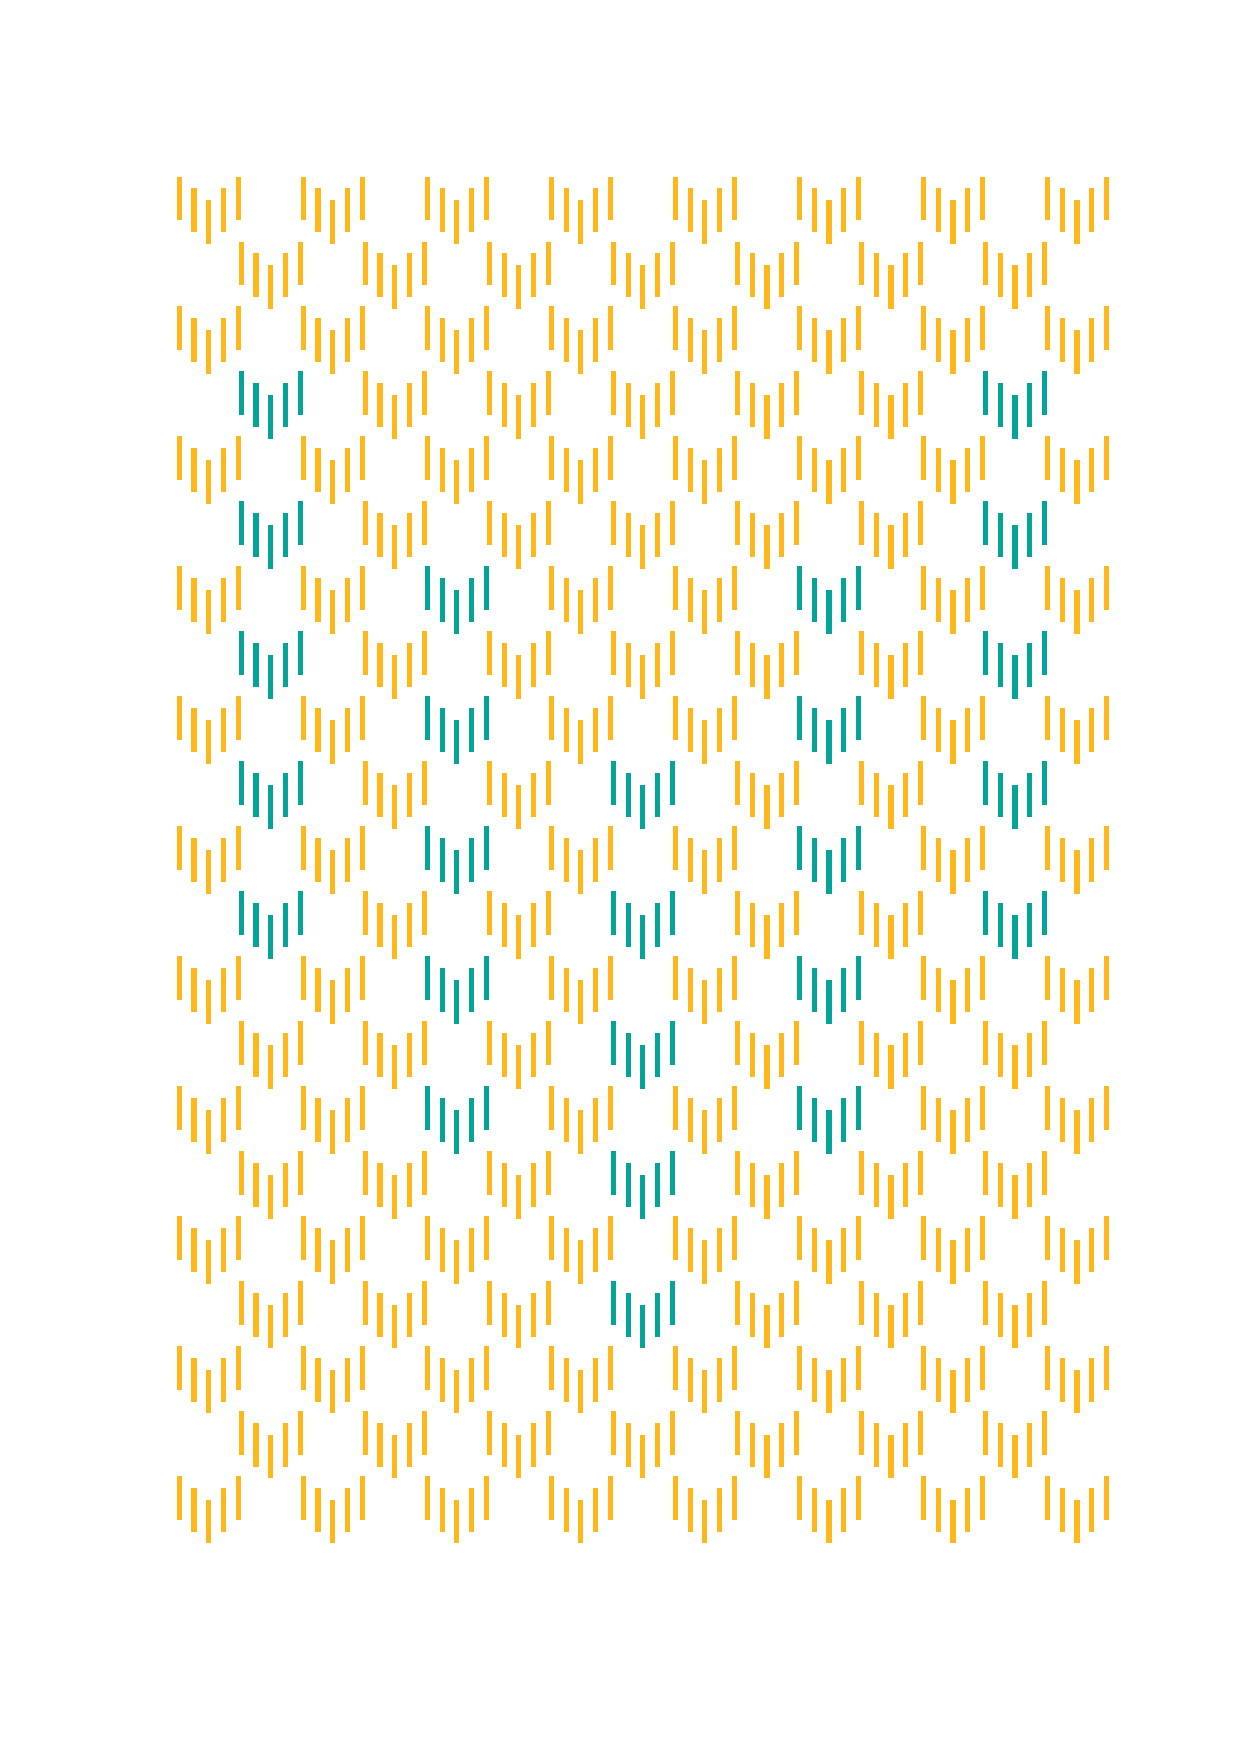
\includepdf[fitpaper=true, pages={1}]{obrazky/uvodv_digital.pdf}
\cleardoublepage

% titulní strana (lícová)
\pagenumbering{roman} % římské číslování stránek
\maketitle
\cleardoublepage

\subfileinclude{kapitoly/biblio_zaznam}

% zadání 
% \includepdf[fitpaper=true, pages={1}]{assignment.pdf} % dle poslední směrnice se zadání nevkládá

\pagestyle{empty}
% \cfoot{}


% prohlášení
% \subfileinclude{kapitoly/prohlaseni} % dle poslední směrnice se prohlášení nevkládá

% obsah 
\thispagestyle{empty}
\tableofcontents
\clearpage

% seznam značek a symbolů
\pagestyle{scrheadings}
\ihead{} % záhlaví - vnitřní
\ohead{} % záhlaví - vnější
\chead{} % záhlaví - střední
\cfoot{} % zápatí
\subfileinclude{kapitoly/seznam_znacek}

\pagenumbering{arabic} % arabské číslování stránek

% úvod
\subfileinclude{kapitoly/uvod}

% kapitoly
% záhlaví/zápatí
\pagestyle{scrheadings}
\rohead{Diplomová práce}
\lehead{\@author}
\chead{}
\cfoot{}
\KOMAoptions{headsepline=0.5pt}

% české uvozovky: „-alt+shift+N, “-alt+shift+H (macOS)

\subfileinclude{kapitoly/kapitola_01}

\subfileinclude{kapitoly/kapitola_02}

% \subfileinclude{kapitoly/kapitola_03}

% \subfileinclude{kapitoly/kapitola_04}

% \subfileinclude{kapitoly/kapitola_05}

% \subfileinclude{kapitoly/kapitola_06}

% \subfileinclude{kapitoly/kapitola_07}

% závěr
\pagestyle{scrheadings}
\ihead{}
\ohead{}
\chead{}
\cfoot{}
\KOMAoptions{headsepline=0pt}

\subfileinclude{kapitoly/zaver}

\subfileinclude{kapitoly/podekovani}


% přílohy

% bibliografie

\bibliographystyle{czechisounsrt}
\bibliography{thesis}
\clearpage


\listoffigures
\clearpage


\listoftables
\clearpage

\addcontentsline{toc}{section}{Seznam příloh}
\section*{Seznam příloh}

\end{document}
\makeatother
